De maneira a verificar o funcionamento do programa, primeiramente testaram-se as funcionalidades deste com o simulador. Para tal apresenta-se de seguida os resultados obtidos para um sinal sinusoidal de $25$Hz, $5$V de amplitude e $0$V de \textit{offset}, e ainda para a variação de uma fonte DC (escala de $5$V/div como pedido).

\begin{figure}[H]
    \centering
    \begin{subfigure}{0.35\textwidth}
        \centering
        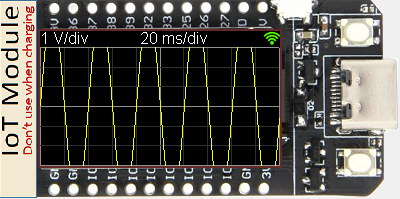
\includegraphics[width=1\linewidth]{Imagens/Testes no simulador/Vertical 1V.png}
        \captionsetup{justification=centering}
        \caption{1V/div e 20ms/div}
        \label{fig:1V/div e 20ms/div simulador}
    \end{subfigure}
    \begin{subfigure}{0.35\textwidth}
        \centering
        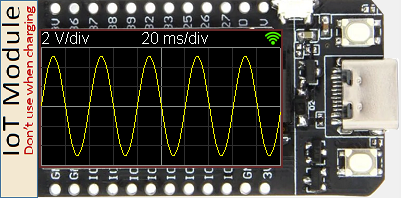
\includegraphics[width=1\linewidth]{Imagens/Testes no simulador/Vertical 2V.png}
        \captionsetup{justification=centering}
        \caption{2V/div e 20ms/div}
        \label{fig:2V/div e 20ms/div simulador}
    \end{subfigure}
    \begin{subfigure}{0.35\textwidth}
        \centering
        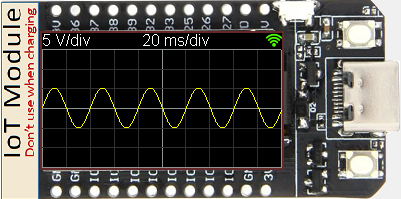
\includegraphics[width=1\linewidth]{Imagens/Testes no simulador/Vertical 5V.png}
        \captionsetup{justification=centering}
        \caption{5V/div e 20ms/div}
        \label{fig:5V/div e 20ms/div simulador}
    \end{subfigure}
    \begin{subfigure}{0.35\textwidth}
        \centering
        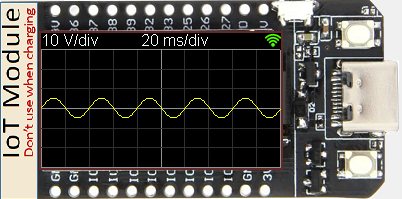
\includegraphics[width=1\linewidth]{Imagens/Testes no simulador/Vertical 10V.png}
        \captionsetup{justification=centering}
        \caption{10V/div e 20ms/div}
        \label{fig:10V/div e 20ms/div vertical simulador}
    \end{subfigure}
    \captionsetup{justification=centering}
    \caption{Variação da escala vertical (simulador)}
    \label{fig:Variação da escala vertical (simulador)}
\end{figure}

\phantom{test}

\vspace{1cm}

\begin{figure}[H]
    \centering
    \begin{subfigure}{0.35\textwidth}
        \centering
        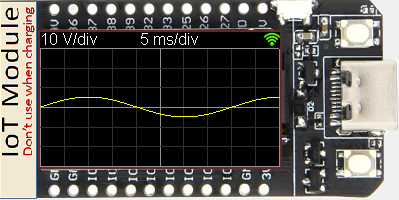
\includegraphics[width=1\linewidth]{Imagens/Testes no simulador/Horizontal 5ms.png}
        \captionsetup{justification=centering}
        \caption{10V/div e 5ms/div}
        \label{fig:10V/div e 5ms/div simulador}
    \end{subfigure}
    \begin{subfigure}{0.35\textwidth}
        \centering
        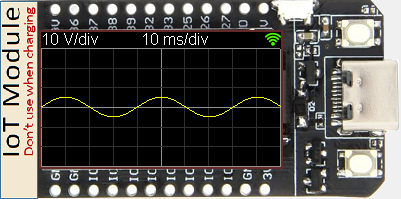
\includegraphics[width=1\linewidth]{Imagens/Testes no simulador/Horizontal 10ms.png}
        \captionsetup{justification=centering}
        \caption{10V/div e 10ms/div}
        \label{fig:10V/div e 10ms/div simulador}
    \end{subfigure}
    \begin{subfigure}{0.35\textwidth}
        \centering
        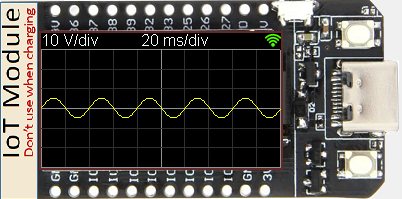
\includegraphics[width=1\linewidth]{Imagens/Testes no simulador/Horizontal 20ms.png}
        \captionsetup{justification=centering}
        \caption{10V/div e 20ms/div}
        \label{fig:10V/div e 20ms/div horizontal simulador}
    \end{subfigure}
    \begin{subfigure}{0.35\textwidth}
        \centering
        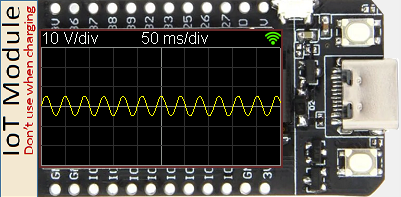
\includegraphics[width=1\linewidth]{Imagens/Testes no simulador/Horizontal 50ms.png}
        \captionsetup{justification=centering}
        \caption{10V/div e 50ms/div}
        \label{fig:10V/div e 50ms/div simulador}
    \end{subfigure}
    \captionsetup{justification=centering}
    \caption{Variação da escala horizontal (simulador)}
    \label{fig:Variação da escala horizontal (simulador)}
\end{figure}

\begin{figure}[H]
    \centering
    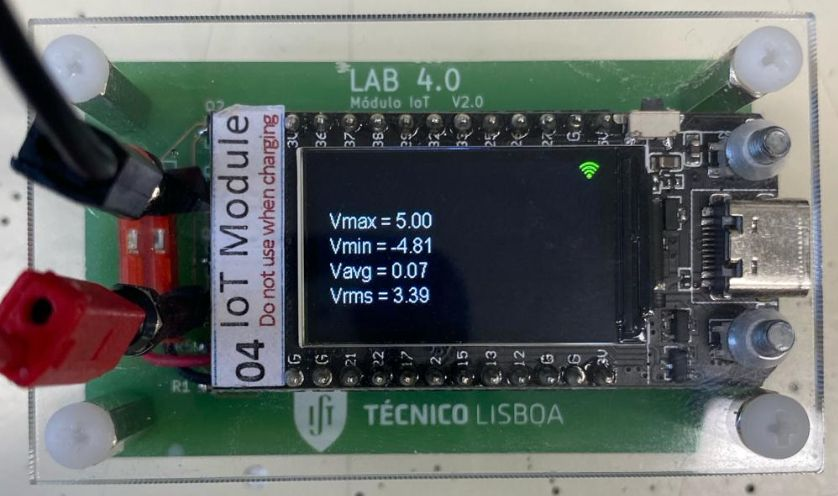
\includegraphics[width=0.35\textwidth]{Imagens/Testes no simulador/Botão 13.png}
    \captionsetup{justification=centering}
    \caption{Funcionamento do duplo clique do botão 1 (simulador)}
    \label{fig:Funcionamento do duplo clique do botão 1 (simulador)}
\end{figure}

\begin{figure}[H]
    \centering
    \begin{subfigure}{0.35\textwidth}
        \centering
        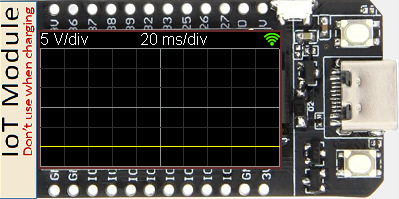
\includegraphics[width=1\linewidth]{Imagens/Testes no simulador/DC -10V.png}
        \captionsetup{justification=centering}
        \caption{DC -10V}
        \label{fig:DC -10V simulador}
    \end{subfigure}
    \begin{subfigure}{0.35\textwidth}
        \centering
        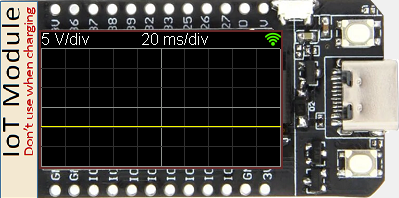
\includegraphics[width=1\linewidth]{Imagens/Testes no simulador/DC -5V.png}
        \captionsetup{justification=centering}
        \caption{DC -5V}
        \label{fig:DC -5V simulador}
    \end{subfigure}
    \begin{subfigure}{0.35\textwidth}
        \centering
        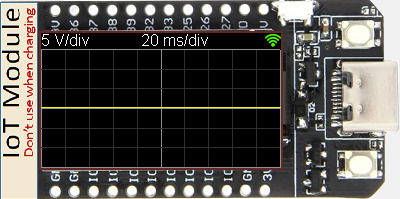
\includegraphics[width=1\linewidth]{Imagens/Testes no simulador/DC 0V.png}
        \captionsetup{justification=centering}
        \caption{DC 0V}
        \label{fig:DC 0V simulador}
    \end{subfigure}
    \begin{subfigure}{0.35\textwidth}
        \centering
        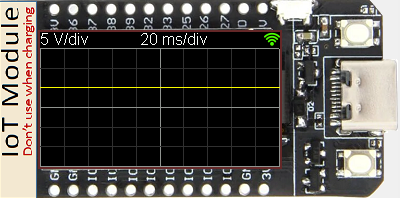
\includegraphics[width=1\linewidth]{Imagens/Testes no simulador/DC 5V.png}
        \captionsetup{justification=centering}
        \caption{DC 5V}
        \label{fig:DC 5V simulador}
    \end{subfigure}
\end{figure}

\begin{figure}[H]\ContinuedFloat
    \centering
    \begin{subfigure}{0.35\textwidth}
        \centering
        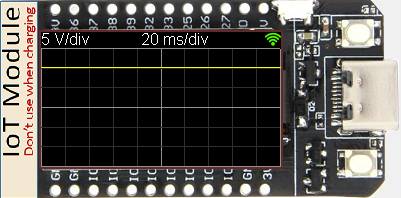
\includegraphics[width=1\linewidth]{Imagens/Testes no simulador/DC 10V.png}
        \captionsetup{justification=centering}
        \caption{DC 10V}
        \label{fig:DC 10V simulador}
    \end{subfigure}
    \captionsetup{justification=centering}
    \caption{Variação de uma tensão DC (simulador)}
    \label{fig:Variação de uma tensão DC (simulador)}
\end{figure}

Aqui não se apresenta a onda quadrada com que o programa tem de ser testado uma vez que o obtido é exatamente igual ao que está no enunciado. A funcionalidade da DFT será demonstrada nos \nameref{sec:Testes no laboratório}.

Como seria de esperar, no simulador com a calibração de origem do Professor verifica-se a correta representação de todos os sinais e funcionalidade do programa desenvolvido. Nos testes experimentais é inevitável que haja erros a nível de ruído e no conjunto de medidas determinado, o que será discutido de seguida.